\documentclass[]{exam}
\usepackage[table]{xcolor}
\usepackage{array}
\usepackage{multirow}
\usepackage{amsmath}
\usepackage{amssymb}
\usepackage{graphicx}
\usepackage{float}
\usepackage[a4paper, total={6in, 9in}]{geometry}
\usepackage[hidelinks]{hyperref}
\usepackage{xepersian}

\settextfont[Path=../../fonts/,AutoFakeBold=2.5]{XB Niloofar.ttf}

\begin{document}
\pagestyle{head}
\firstpageheader{}{}{}
\runningheader{صفحه \thepage\ از \numpages}{}{}
\runningheadrule

\begin{tabular}{p{.75\textwidth} l}
\multicolumn{2}{c}{\textbf{به نام خدا}}\\
\multirow{2}{*}{
\includegraphics[scale=0.2] {../../assets/ui-logo.png}} & \\ \\
&  \textbf{علوم کامپیوتر}\\
&  \textbf{نیم‌سال دوم ۰۴-۰۵}\\
&  \textbf{داده کاوی}\\ \\
 \textbf{دانشکده ریاضی و آمار} &  \\
\end{tabular}\\
\noindent\rule{\textwidth}{0.5pt}

\vspace{0.1cm}

\textbf{زهرا چراغی، محمد ملائی، داوود نصرتی}

\noindent\rule{\textwidth}{0.5pt}

\section*{صورت سؤال}

در یک مسئله‌ی پزشکی، یک سیستم تشخیص بیماری دیابت داریم. حساسیت سیستم برابر با \(0.80\) و ویژگی آن برابر با \(0.95\) است. می‌خواهیم احتمال این را محاسبه کنیم که سیستم خروجی «داشتن دیابت» بدهد، اما فرد واقعاً دیابت نداشته باشد. این محاسبه یک بار بر اساس شیوع گزارش‌شده در مقاله و یک بار بر اساس فرض خود سؤال، یعنی شیوع \(10\%\)، انجام می‌شود.

\section*{مقدمه}

احتمال مورد نظر برابر است با احتمال اینکه خروجی سیستم مثبت باشد، اما فرد در واقع دیابت نداشته باشد.

این مقدار همان نرخ کشف کاذب یا \lr{False Discovery Rate} است. از طرف دیگر، ارزش اخباری مثبت یا \lr{Positive Predictive Value} نشان می‌دهد که چه نسبتی از خروجی‌های مثبت سیستم واقعاً بیمار هستند.

پس داریم:

\[
FDR = 1 - PPV
\]

برای محاسبه‌ی \(PPV\)، از رابطه‌ی زیر استفاده می‌کنیم:

\[
PPV =
\frac{Se \times Prevalence}
{(Se \times Prevalence) + (1-Sp)\times(1-Prevalence)}
\]

\section*{۱. محاسبه بر اساس مقاله}

مقاله‌ی استفاده‌شده با عنوان زیر است:

\begin{center}
\lr{\textit{The prevalence of impaired fasting glucose and type 2 diabetes in a population-based sample of overweight/obese children in the Middle East}}
\end{center}

آدرس مقاله:

\begin{center}
\href{https://pubmed.ncbi.nlm.nih.gov/19765232/}{\lr{https://pubmed.ncbi.nlm.nih.gov/19765232/}}
\end{center}

\begin{figure}[H]
\centering
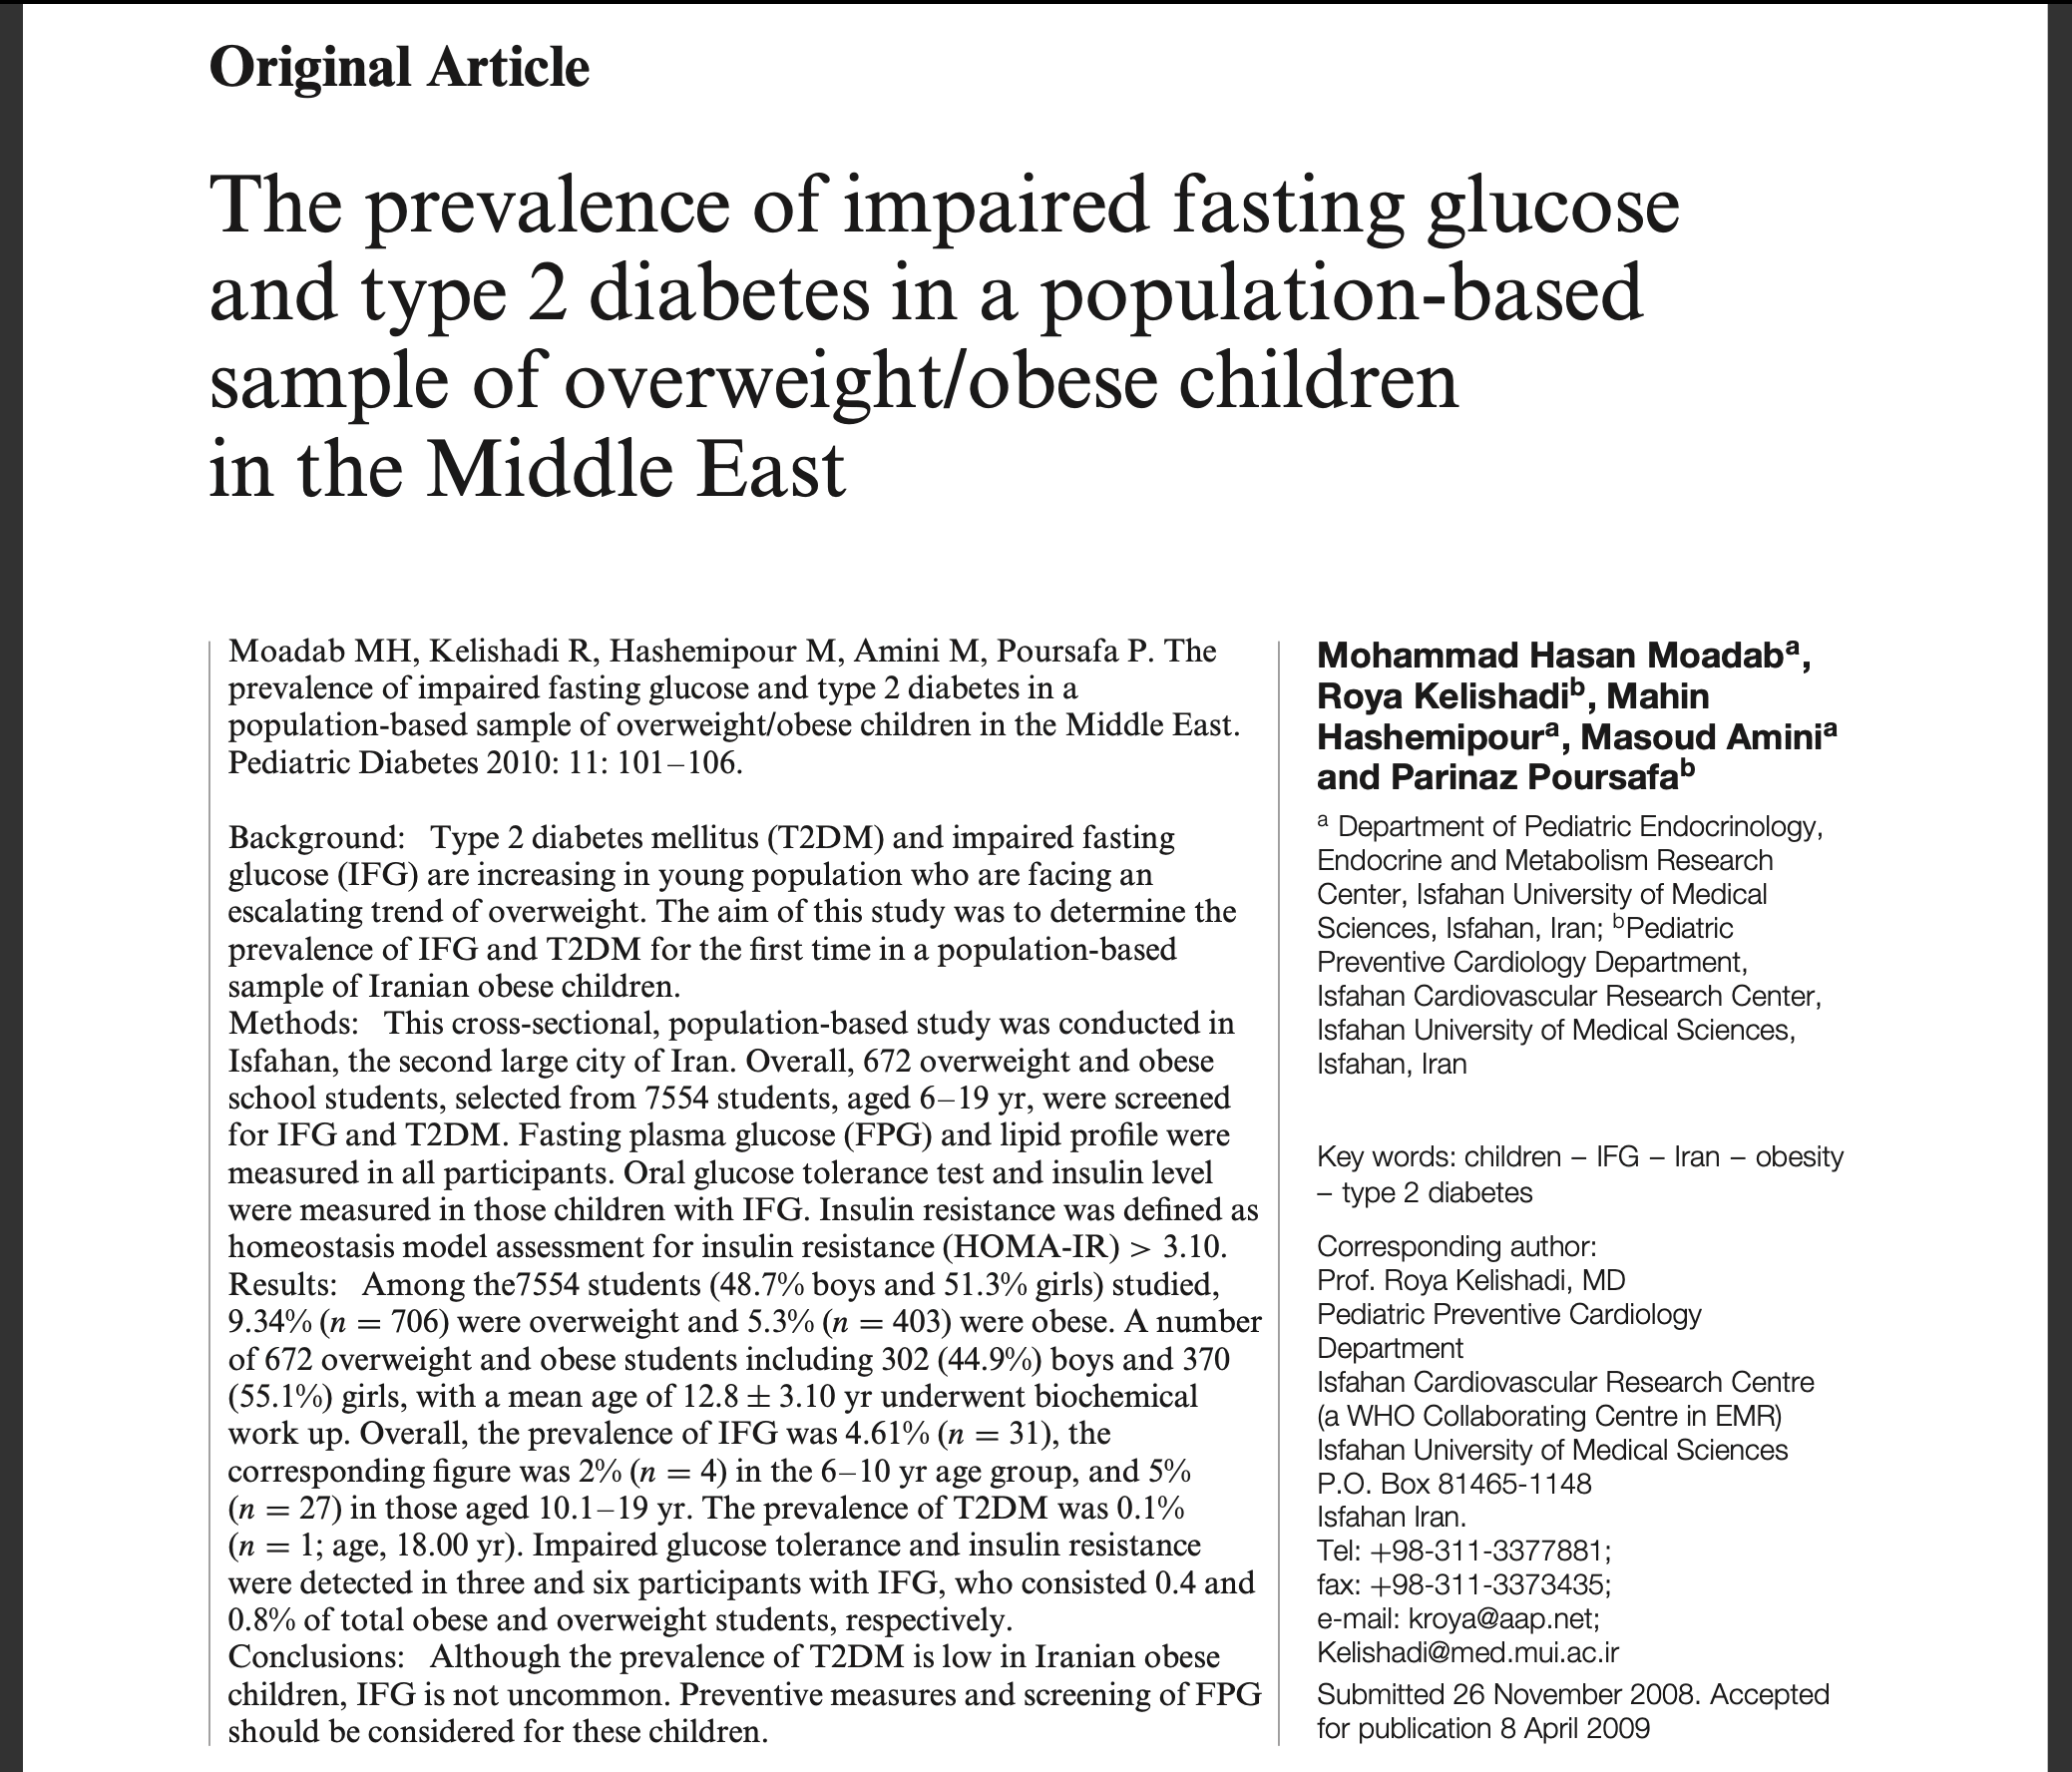
\includegraphics[width=0.95\textwidth]{figures/article-first-page.png}
\caption{صفحه‌ی اول مقاله‌ی مورد استفاده برای استخراج شیوع دیابت نوع ۲}
\end{figure}

همان‌طور که در تصویر مقاله دیده می‌شود، این مطالعه در شهر اصفهان و روی دانش‌آموزان \(6\) تا \(19\) ساله‌ی دارای اضافه‌وزن یا چاقی انجام شده است. در بخش نتایج مقاله، شیوع دیابت نوع ۲ در این گروه برابر با \(0.1\%\) گزارش شده است. بنابراین اگر جامعه‌ی هدف را همین گروه در نظر بگیریم، مقدار شیوع برابر است با:

\[
Prevalence = 0.1\% = 0.001
\]

داده‌ها:

\[
Se = 0.80
\]

\[
Sp = 0.95
\]

\[
Prevalence = 0.001
\]

پس:

\[
FDR = 1 - PPV
\]

\[
FDR =
1 -
\frac{0.8 \times 0.001}
{(0.8 \times 0.001) + (1-0.95)\times(1-0.001)}
\]

\[
FDR =
1 -
\frac{0.0008}
{0.0008 + 0.05 \times 0.999}
\]

\[
FDR =
1 -
\frac{0.0008}
{0.0008 + 0.04995}
\]

\[
FDR =
1 -
\frac{0.0008}{0.05075}
\]

\[
FDR \approx 1 - 0.01576
\]

\[
FDR \approx 0.98424
\]

بنابراین، بر اساس شیوع گزارش‌شده در مقاله:

\[
\boxed{FDR \approx 98.42\%}
\]

یعنی اگر از شیوع \(0.1\%\) گزارش‌شده در مقاله استفاده کنیم، احتمال اینکه سیستم خروجی «داشتن دیابت» بدهد ولی فرد واقعاً دیابت نداشته باشد، حدود \(98.42\%\) است.

\section*{۲. محاسبه بر اساس فرض سؤال}

اگر طبق صورت سؤال، شیوع دیابت برابر با \(10\%\) فرض شود، داریم:

\[
Prevalence = 10\% = 0.10
\]

داده‌ها:

\[
Se = 0.80
\]

\[
Sp = 0.95
\]

\[
Prevalence = 0.10
\]

پس:

\[
FDR =
1 -
\frac{0.8 \times 0.10}
{(0.8 \times 0.10) + (1-0.95)\times(1-0.10)}
\]

\[
FDR =
1 -
\frac{0.08}
{0.08 + 0.05 \times 0.90}
\]

\[
FDR =
1 -
\frac{0.08}
{0.08 + 0.045}
\]

\[
FDR =
1 -
\frac{0.08}{0.125}
\]

\[
FDR = 1 - 0.64
\]

\[
FDR = 0.36
\]

بنابراین، بر اساس فرض خود سؤال:

\[
\boxed{FDR = 36\%}
\]

یعنی اگر شیوع دیابت در جامعه یا دیتاست مورد نظر سؤال برابر با \(10\%\) باشد، احتمال اینکه سیستم خروجی «داشتن دیابت» بدهد ولی فرد واقعاً دیابت نداشته باشد، برابر با \(36\%\) است.

\section*{نتیجه نهایی}

اگر سؤال صراحتاً شیوع را \(10\%\) داده باشد، پاسخ نهایی باید برابر با \(36\%\) باشد:

\[
\boxed{36\%}
\]

اما اگر بخواهیم محاسبه را بر اساس شیوع گزارش‌شده در مقاله، یعنی \(0.1\%\)، انجام دهیم، مقدار به دست آمده برابر است با:

\[
\boxed{98.42\%}
\]

\end{document}
